\chapter{One-dimensional Integrals in Several Variables} \label{path:chapter}

%%%%%%%%%%%%%%%%%%%%%%%%%%%%%%%%%%%%%%%%%%%%%%%%%%%%%%%%%%%%%%%%%%%%%%%%%%%%%%

\section{Differentiation under the integral}
\label{sec:diffunderint}

\sectionnotes{less than 1 lecture}

Let $f(x,y)$ be a function of two variables and define
\begin{equation*}
g(y) := \int_a^b f(x,y) ~dx .
\end{equation*}
If $f$ is continuous on the compact rectangle $[a,b] \times [c,d]$, then
\volIref{\propref*{vI-prop:integralcontcont} from volume I}{\propref{prop:integralcontcont}}
says that $g$ is continuous on $[c,d]$.

Suppose $f$ is differentiable in $y$.  The main question we want to
ask is when can we \myquote{differentiate under the integral,} that is,
when is it true that $g$ is differentiable and its derivative is
\begin{equation*}
g'(y) \overset{?}{=} \int_a^b \frac{\partial f}{\partial y}(x,y) ~dx .
\end{equation*}
Differentiation is a limit and therefore we are really asking when do the
two limiting operations of integration and differentiation commute.
This is not always possible and some extra hypothesis is
necessary.  The first
question we would face is the integrability of
$\frac{\partial f}{\partial y}$, but the formula above can fail even if
$\frac{\partial f}{\partial y}$ is integrable as a function of $x$ for every
fixed $y$.

We prove a simple, but perhaps the most useful version of this kind of result.

\begin{thm}[\myindex{Leibniz integral rule}]
Suppose $f \colon [a,b] \times [c,d] \to \R$ is a continuous function,
such that $\frac{\partial f}{\partial y}$ exists for all $(x,y) \in [a,b]
\times [c,d]$ and is continuous.  Define
\begin{equation*}
g(y) := \int_a^b f(x,y) ~dx .
\end{equation*}
Then $g \colon [c,d] \to \R$ is continuously differentiable and
\begin{equation*}
g'(y) = \int_a^b \frac{\partial f}{\partial y}(x,y) ~dx .
\end{equation*}
\end{thm}

The hypotheses on $f$ and $\frac{\partial f}{\partial y}$ can be
weakened, see e.g.\ \exerciseref{exercise:strongerleibniz},
but not dropped outright.
The main point in the proof requires that
$\frac{\partial f}{\partial y}$ exists and is continuous for all $x$
up to the endpoints, but we only need a small
interval in the $y$ direction.  In applications, we often make $[c,d]$ a
small interval around the point where we need to differentiate.

\begin{proof}
Fix $y \in [c,d]$ and let $\epsilon > 0$ be given.
As $\frac{\partial f}{\partial y}$ is continuous on $[a,b] \times [c,d]$ it
is uniformly continuous.  In particular, there exists $\delta > 0$ such that
whenever $y_1 \in [c,d]$ with
$\abs{y_1-y} < \delta$ and all $x \in [a,b]$ we have
\begin{equation*}
\abs{\frac{\partial f}{\partial y}(x,y_1)-\frac{\partial f}{\partial y}(x,y)} < \epsilon .
\end{equation*}

Suppose $h$ is such that $y+h \in [c,d]$ and $\abs{h} < \delta$.
Fix $x$ for a moment
and apply the mean value theorem to find a $y_1$ between $y$ and $y+h$ such that
\begin{equation*}
\frac{f(x,y+h)-f(x,y)}{h}
=
\frac{\partial f}{\partial y}(x,y_1) .
\end{equation*}
As $\abs{y_1-y} \leq \abs{h} < \delta$,
\begin{equation*}
\abs{
\frac{f(x,y+h)-f(x,y)}{h}
-
\frac{\partial f}{\partial y}(x,y) 
}
=
\abs{
\frac{\partial f}{\partial y}(x,y_1) 
-
\frac{\partial f}{\partial y}(x,y) 
}
< \epsilon .
\end{equation*}
This argument worked for every $x \in [a,b]$.  Therefore, as a function of
$x$
\begin{equation*}
x \mapsto \frac{f(x,y+h)-f(x,y)}{h}
\qquad
\text{converges uniformly to}
\qquad
x \mapsto \frac{\partial f}{\partial y}(x,y)
\qquad
\text{as } h \to 0 .
\end{equation*}
We defined uniform convergence for sequences although the idea is the
same.  You may replace $h$ with a sequence of nonzero 
numbers $\{ h_n \}$
converging to $0$ such that $y+h_n \in [c,d]$ and let $n \to \infty$.

Consider the difference quotient of $g$,
\begin{equation*}
\frac{g(y+h)-g(y)}{h}
=
\frac{\int_a^b f(x,y+h) ~dx -
\int_a^b f(x,y) ~dx }{h}
=
\int_a^b \frac{f(x,y+h)-f(x,y)}{h} ~dx .
\end{equation*}
Uniform convergence implies the limit can be taken underneath the integral.
So
\begin{equation*}
\lim_{h\to 0}
\frac{g(y+h)-g(y)}{h}
= 
\int_a^b 
\lim_{h\to 0}
\frac{f(x,y+h)-f(x,y)}{h} ~dx 
=
\int_a^b 
\frac{\partial f}{\partial y}(x,y) ~dx .
\end{equation*}
Then $g'$ is continuous on $[c,d]$ by
\volIref{\propref*{vI-prop:integralcontcont} from volume I}{\propref{prop:integralcontcont}} mentioned above.
\end{proof}

\begin{example}
Let
\begin{equation*}
f(y) = \int_0^1 \sin(x^2-y^2) ~dx .
\end{equation*}
Then
\begin{equation*}
f'(y) = \int_0^1 -2y\cos(x^2-y^2) ~dx .
\end{equation*}
\end{example}

\begin{example} \label{example:counterexamplediffunder}
Consider
\begin{equation*}
\int_0^{1} \frac{x-1}{\ln(x)} ~dx .
\end{equation*}
The function under the integral 
extends to be continuous on $[0,1]$, and hence
the integral exists, see \exerciseref{exercise:counterexamplediffunder}.  Trouble is finding it.  Introduce a parameter $y$
and define a function:
\begin{equation*}
g(y) := \int_0^{1} \frac{x^y-1}{\ln(x)} ~dx .
\end{equation*}
The function
$\frac{x^y-1}{\ln(x)}$
also extends to a continuous function of $x$ and $y$
for $(x,y) \in [0,1] \times [0,1]$ (also in the exercise).
See \figureref{fig:diffunderexample}.
\begin{myfigureht}
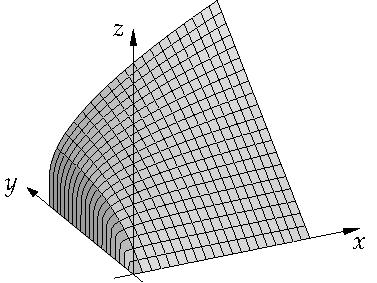
\includegraphics{figures/diffunderexample}
\caption{The graph $z= \frac{x^y-1}{\ln(x)}$ on $[0,1] \times [0,1]$.\label{fig:diffunderexample}}
\end{myfigureht}


Hence,
$g$ is a continuous function on $[0,1]$ and $g(0) = 0$.
For any $\epsilon > 0$, the $y$ derivative of the integrand, $x^y$,
is continuous on $[0,1] \times [\epsilon,1]$.  Therefore,
for $y >0$, we may differentiate under the integral sign
\begin{equation*}
g'(y) =
\int_0^{1} \frac{\ln(x) x^y}{\ln(x)} ~dx 
=
\int_0^{1} x^y ~dx =
\frac{1}{y+1} .
\end{equation*}
We need to figure out $g(1)$ given that $g'(y) = \frac{1}{y+1}$ and $g(0) =
0$.  Elementary calculus says that $g(1) = \int_0^1 g'(y)~dy = \ln(2)$.
Thus,
\begin{equation*}
\int_0^{1} \frac{x-1}{\ln(x)} ~dx  = \ln(2).
\end{equation*}
\end{example}

\subsection{Exercises}

\begin{exercise} \label{exercise:counterexamplediffunder}
Prove the two statements that were asserted in
\exampleref{example:counterexamplediffunder}:
\begin{enumerate}[a)]
\item
Prove $\frac{x-1}{\ln(x)}$ extends to a continuous function of
$[0,1]$.  That is, there exists a continuous function on $[0,1]$
that equals $\frac{x-1}{\ln(x)}$ on $(0,1)$.
\item
Prove $\frac{x^y-1}{\ln(x)}$ extends to a continuous function
on $[0,1] \times [0,1]$.
\end{enumerate}
\end{exercise}

\begin{exercise}
Suppose $h \colon \R \to \R$ is continuous and $g
\colon \R \to \R$ is continuously differentiable and compactly
supported.  That is, there exists some $M > 0$, such that $g(x) = 0$ whenever
$\abs{x} \geq M$.  Define
\begin{equation*}
f(x) := \int_{-\infty}^\infty h(y)g(x-y)~dy  .
\end{equation*}
Show that $f$ is differentiable.
\end{exercise}

\begin{exercise}
Suppose $f \colon \R \to \R$ is infinitely differentiable (all derivatives exist)
such that $f(0) = 0$.  Then show that there exists an infinitely
differentiable function $g \colon \R \to \R$ such that $f(x) = x\,g(x)$.
Show also that
if $f'(0) \not= 0$, then $g(0) \not= 0$.\\
Hint: First write
$f(x) = \int_0^x f'(s) ~ds$ and then rewrite the integral to go
from $0$ to $1$.
\end{exercise}


\begin{exercise}
Compute $\int_0^1 e^{tx} ~dx$.  Derive the formula for
$\int_0^1 x^n e^{x} ~dx$ not using integration by parts, but
by differentiation underneath the integral.
\end{exercise}

\begin{exercise}
Let $U \subset \R^n$ be an open set and suppose
$f(x,y_1,y_2,\ldots,y_n)$ is a continuous
function defined on $[0,1] \times U \subset \R^{n+1}$.
Suppose
$\frac{\partial f}{\partial y_1},
\frac{\partial f}{\partial y_2},\ldots,
\frac{\partial f}{\partial y_n}$
exist and are continuous on $[0,1] \times U$.
Then prove that $F \colon U \to \R$ defined by
\begin{equation*}
F(y_1,y_2,\ldots,y_n) :=
\int_0^1
f(x,y_1,y_2,\ldots,y_n)
~ dx
\end{equation*}
is continuously differentiable.
\end{exercise}

\begin{exercise}
Work out the following counterexample:  Let
\begin{equation*}
f(x,y) :=
\begin{cases}
\frac{xy^3}{{(x^2+y^2)}^2} & \text{if } x\not=0 \text{ or } y\not= 0, \\
0                          & \text{if } x=0 \text{ and } y=0.
\end{cases}
\end{equation*}
\begin{enumerate}[a)]
\item
Prove that for any fixed $y$ the function $x \mapsto f(x,y)$ is
Riemann integrable on $[0,1]$ and
\begin{equation*}
g(y) := \int_0^1 f(x,y) ~ dx = \frac{y}{2y^2+2} .
\end{equation*}
Therefore, $g'(y)$ exists and its derivative is the continuous function
\begin{equation*}
g'(y) =
\frac{d}{dy} \int_0^1 f(x,y) ~ dx
=
\frac{1-y^2}{2{(y^2+1)}^2} .
\end{equation*}
\item
Prove $\frac{\partial f}{\partial y}$ exists at all $x$ and $y$ and
compute it.
\item
Show that for all $y$
\begin{equation*}
\int_0^1 \frac{\partial f}{\partial y} (x,y) ~ dx
\end{equation*}
exists, but
\begin{equation*}
g'(0) \not= \int_0^1 \frac{\partial f}{\partial y} (x,0) ~ dx .
\end{equation*}
\end{enumerate}
\end{exercise}

\pagebreak[2]
\begin{exercise}
Work out the following counterexample:  Let
\begin{equation*}
f(x,y) :=
\begin{cases}
x \,\sin \left(\frac{y}{x^2+y^2}\right) & \text{if } (x,y) \not= (0,0),\\
0                                       & \text{if } (x,y)=(0,0).
\end{cases}
\end{equation*}
\begin{enumerate}[a)]
\item
Prove $f$ is continuous on all of $\R^2$.
Therefore the following function is well-defined for every $y \in \R$:
\begin{equation*}
g(y) := \int_0^1 f(x,y) ~ dx .
\end{equation*}
\item
Prove $\frac{\partial f}{\partial y}$ exists for all $(x,y)$,
but is not continuous at $(0,0)$.
\item
Show that $\int_0^1 \frac{\partial f}{\partial y}(x,0) ~ dx$ does not
exist even if we take improper integrals, that is,
that the limit
$\lim\limits_{h \to 0^+} \int_h^1 \frac{\partial f}{\partial y}(x,0) ~ dx$
does not exist.
\end{enumerate}
Note: Feel free to use what you know about sine and cosine from calculus.
\end{exercise}

\begin{exercise} \label{exercise:strongerleibniz}
Strengthen the Leibniz integral rule in the following way.
Suppose $f \colon (a,b) \times (c,d) \to \R$ is a bounded continuous function,
such that $\frac{\partial f}{\partial y}$ exists for all $(x,y) \in (a,b)
\times (c,d)$ and is continuous and bounded.  Define
\begin{equation*}
g(y) := \int_a^b f(x,y) ~dx .
\end{equation*}
Then $g \colon (c,d) \to \R$ is continuously differentiable and
\begin{equation*}
g'(y) = \int_a^b \frac{\partial f}{\partial y}(x,y) ~dx .
\end{equation*}
Hint: See also \volIref{\exerciseref*{vI-exercise:integralcontcontextra} and
\thmref*{vI-thm:dersconverge} from
volume I}{\exerciseref{exercise:integralcontcontextra} and
\thmref{thm:dersconverge}}.
\end{exercise}

%%%%%%%%%%%%%%%%%%%%%%%%%%%%%%%%%%%%%%%%%%%%%%%%%%%%%%%%%%%%%%%%%%%%%%%%%%%%%%

\sectionnewpage
\section{Path integrals}
\label{sec:pathintegral}

\sectionnotes{2--3 lectures}

\subsection{Piecewise smooth paths}

Let $\gamma \colon [a,b] \to \R^n$ be a function and write
$\gamma = (\gamma_1,\gamma_2,\ldots,\gamma_n)$. 
Suppose $\gamma$ is 
\emph{continuously differentiable},
that is,
it is differentiable and the derivative is continuous.
In other words, there exists a continuous function $\gamma^{\:\prime} \colon [a,b]
\to \R^n$ such that for every $t \in [a,b]$, we have
$\lim\limits_{h \to 0}
\frac{\snorm{\gamma(t+h)-\gamma(t) - \gamma^{\:\prime}(t) \, h}}{\sabs{h}} = 0$.
We treat
$\gamma^{\:\prime}(t)$ either as a linear operator (an $n \times 1$ matrix) or
a vector,
$\gamma^{\:\prime}(t) =
\bigl( \gamma_1^{\:\prime}(t), \gamma_2^{\:\prime}(t), \ldots,
\gamma_n^{\:\prime}(t) \bigr)$.
Equivalently, 
$\gamma_j$ is a continuously differentiable function on $[a,b]$
for every $j=1,2,\ldots,n$.
By \exerciseref{exercise:normonedim}, the operator norm of
the operator $\gamma^{\:\prime}(t)$ is equal to
the euclidean norm of the corresponding vector, so there is no
confusion when writing $\snorm{\gamma^{\:\prime}(t)}$.

\begin{defn}
A continuously differentiable function $\gamma \colon [a,b] \to \R^n$ is
called a \emph{\myindex{smooth path}}
or a
\emph{\myindex{continuously differentiable path}}\footnote{The
word \myquote{smooth} can sometimes mean
\myquote{infinitely differentiable} in the literature.}
if
$\gamma$ is continuously differentiable and
$\gamma^{\:\prime}(t) \not= 0$ for all $t \in [a,b]$.

The function $\gamma \colon [a,b] \to \R^n$ is called a
\emph{\myindex{piecewise smooth path}} or a
\emph{\myindex{piecewise continuously differentiable path}}
if there exist finitely many points
$t_0 = a < t_1 < t_2 < \cdots < t_k = b$ such that
the restriction $\gamma|_{[t_{j-1},t_j]}$ is smooth path for every
$j=1,2,\ldots,k$.

A path $\gamma$ is 
a \emph{\myindex{closed path}} if $\gamma(a) = \gamma(b)$, that is
if the path starts and ends in the same point.
A path $\gamma$ is a \emph{\myindex{simple path}} if 
either 1) $\gamma$ is a one-to-one function, or 2)
$\gamma|_{[a,b)}$ is one-to-one and $\gamma(a)=\gamma(b)$ ($\gamma$ is a
simple closed path).
\end{defn}


\begin{example} \label{mv:example:unitsquarepath}
Let $\gamma \colon [0,4] \to \R^2$ be defined by
\begin{equation*}
\gamma(t) :=
\begin{cases}
(t,0)   & \text{if } t \in [0,1],\\
(1,t-1) & \text{if } t \in (1,2],\\
(3-t,1) & \text{if } t \in (2,3],\\
(0,4-t) & \text{if } t \in (3,4].
\end{cases}
\end{equation*}
\begin{myfigureht}
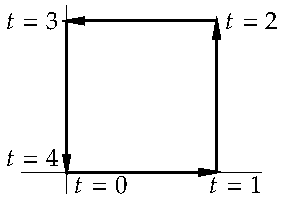
\includegraphics{figures/squarepath}
\caption{The path $\gamma$ traversing the unit square.\label{fig:squarepath}}
\end{myfigureht}

The path $\gamma$ is the unit square traversed
counterclockwise.  See \figureref{fig:squarepath}.  It is
a piecewise smooth path.  For example,
$\gamma|_{[1,2]}(t) = (1,t-1)$ and so
$(\gamma|_{[1,2]})'(t) = (0,1) \not= 0$.  Similarly for the other 3 sides.
Notice
that
$(\gamma|_{[1,2]})'(1) = (0,1)$,
$(\gamma|_{[0,1]})'(1) = (1,0)$, but
$\gamma^{\:\prime}(1)$ does not exist.  At the corners $\gamma$ is 
not differentiable.
The path $\gamma$ is a simple closed path, as $\gamma|_{[0,4)}$ is
one-to-one and $\gamma(0)=\gamma(4)$.
\end{example}

The definition of a piecewise smooth path as we have given it implies
continuity (exercise).  For general functions, many authors also
allow finitely many discontinuities, when they use the term \emph{piecewise
smooth}, and so one may say that we defined a piecewise smooth path
to be a \emph{\myindex{continuous piecewise smooth}} function.
While one may get by with smooth paths, for computations, the simplest
paths to write down are often piecewise smooth.

Generally, we are interested in the direct image $\gamma\bigl([a,b]\bigr)$,
rather than the specific parametrization, although that is also
important to some degree.  When we informally talk about a path or a curve,
we often mean the set $\gamma\bigl([a,b]\bigr)$, depending
on context.


\begin{example}
The condition $\gamma^{\:\prime}(t) \not= 0$ means that the image
$\gamma\bigl([a,b]\bigr)$
has no \myquote{corners} where $\gamma$ is smooth.
Consider 
\begin{equation*}
\gamma(t) :=
\begin{cases}
(t^2,0) & \text{if } t < 0,\\
(0,t^2) & \text{if } t \geq 0.
\end{cases}
\end{equation*}
See \figureref{fig:cornersmoothpath}.
It is left for the reader to check that $\gamma$ is continuously
differentiable, yet the image $\gamma(\R) = \bigl\{ (x,y) \in \R^2 : (x,y) =
(s,0) \text{ or } (x,y) = (0,s) \text{ for some } s \geq 0 \bigr\}$ has a
\myquote{corner} at the origin.  And that is because $\gamma^{\:\prime}(0) = (0,0)$.
More complicated examples with, say, infinitely many corners exist,
see the exercises.
\begin{myfigureht}
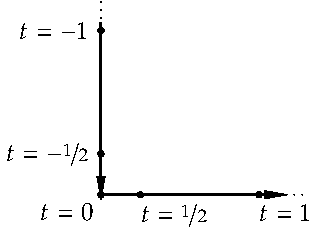
\includegraphics{figures/cornersmoothpath}
\caption{Smooth path with zero derivative with a corner.  Several values of
$t$ are marked with dots.\label{fig:cornersmoothpath}}
\end{myfigureht}
\end{example}

The condition $\gamma^{\:\prime}(t) \not= 0$ even at the endpoints guarantees
not only no corners, but also that the path ends nicely, that is, it can
extend a little bit past the endpoints.  Again, see the exercises.

\begin{example}
A graph of a continuously differentiable function $f \colon [a,b] \to \R$ is a smooth path.
Define $\gamma \colon [a,b] \to \R^2$ by
\begin{equation*}
\gamma(t) := \bigl(t,f(t)\bigr) .
\end{equation*}
Then $\gamma^{\:\prime}(t) = \bigl( 1 , f'(t) \bigr)$, which is never zero,
and $\gamma\bigl([a,b]\bigr)$ is the graph of $f$.

There are other ways of parametrizing the path.  That is, there are
different paths with the same image.
The function $t \mapsto (1-t)a+tb$, takes the interval $[0,1]$ to $[a,b]$.
Define
$\alpha \colon [0,1] \to \R^2$ by
\begin{equation*}
\alpha(t) := \bigl((1-t)a+tb,f((1-t)a+tb)\bigr) .
\end{equation*}
Then
$\alpha'(t) = \bigl( b-a ,~ (b-a)f'((1-t)a+tb) \bigr)$, which is never zero.
As sets, $\alpha\bigl([0,1]\bigr) = \gamma\bigl([a,b]\bigr)
= \bigl\{ (x,y) \in \R^2 : x \in [a,b] \text{ and } f(x) = y \bigr\}$,
which is just the graph of $f$.
\end{example}

The last example leads us to a definition.

\begin{defn}
Let $\gamma \colon [a,b] \to \R^n$ be a smooth path and
$h \colon [c,d] \to [a,b]$ a continuously differentiable bijective function
such that $h'(t) \not= 0$ for all $t \in [c,d]$.  Then
the composition
$\gamma \circ h$ is called a
\emph{\myindex{smooth reparametrization}}\index{reparametrization}
of $\gamma$.

Let $\gamma$ be a piecewise smooth path, and
$h$ a piecewise smooth bijective function with
nonzero one-sided limits of $h'$.
The composition
$\gamma \circ h$ is called a
\emph{\myindex{piecewise smooth reparametrization}} of $\gamma$.

If $h$ is strictly increasing, then $h$ is 
said to \emph{\myindex{preserve orientation}}.  If $h$ does not preserve
orientation, then $h$ is said to \emph{\myindex{reverse orientation}}.
\end{defn}

A reparametrization is another path for the same set.  That is,
$(\gamma \circ h)\bigl([c,d]\bigr) =
\gamma \bigl([a,b]\bigr)$.

The conditions on the piecewise smooth $h$ mean that
there is some partition $t_0 = c < t_1 < t_2 < \cdots < t_k = d$,
such that $h|_{[t_{j-1},t_j]}$ is continuously differentiable
and $(h|_{[t_{j-1},t_j]})'(t) \not= 0$ for all $t \in [t_{j-1},t_j]$.
Since $h$ is bijective, it is either strictly increasing or
strictly decreasing.  So either $(h|_{[t_{j-1},t_j]})'(t) > 0$
for all $t$ or $(h|_{[t_{j-1},t_j]})'(t) < 0$ for all $t$.

\begin{prop} \label{prop:reparamapiecewisesmooth}
If $\gamma \colon [a,b] \to \R^n$ is a piecewise smooth path,
and $\gamma \circ h \colon [c,d] \to \R^n$ is
a piecewise smooth reparametrization, then $\gamma \circ h$
is a piecewise smooth path.
\end{prop}

\begin{proof}
Assume that $h$ preserves orientation, that is, $h$ is strictly
increasing.
If $h \colon [c,d] \to [a,b]$ gives a piecewise smooth reparametrization,
then for some partition
$r_0 = c < r_1 < r_2 < \cdots < r_\ell = d$, the restriction
$h|_{[r_{j-1},r_j]}$ is continuously differentiable with a positive
derivative.

Let $t_0 = a < t_1 < t_2 < \cdots < t_k = b$ be the partition from the
definition of piecewise smooth for $\gamma$ together with the 
points $\{ h(r_0), h(r_1), h(r_2), \ldots, h(r_\ell) \}$.
Let $s_j := h^{-1}(t_j)$.  Then
$s_0 = c < s_1 < s_2 < \cdots < s_k = d$
is a partition that includes (is a refinement of) the
$\{ r_0,r_1,\ldots,r_\ell \}$.
If $\tau \in [s_{j-1},s_j]$, then $h(\tau) \in [t_{j-1},t_j]$
since $h(s_{j-1}) = t_{j-1}$,
$h(s_{j}) = t_j$, and
$h$ is strictly increasing.
Also $h|_{[s_{j-1},s_j]}$ is continuously differentiable, and
$\gamma|_{[t_{j-1},t_j]}$ is also continuously differentiable.
Then
\begin{equation*}
(\gamma \circ h)|_{[s_{j-1},s_{j}]} (\tau)
=
\gamma|_{[t_{j-1},t_{j}]} \bigl( h|_{[s_{j-1},s_j]}(\tau) \bigr) .
\end{equation*}
The function 
$(\gamma \circ h)|_{[s_{j-1},s_{j}]}$ is therefore continuously
differentiable and
by the chain rule
\begin{equation*}
\bigl( (\gamma \circ h)|_{[s_{j-1},s_{j}]} \bigr) ' (\tau)
=
\bigl( \gamma|_{[t_{j-1},t_{j}]} \bigr)' \bigl( h(\tau) \bigr)
(h|_{[s_{j-1},s_j]})'(\tau) \not= 0 .
\end{equation*}
Consequently, $\gamma \circ h$ is a piecewise smooth path.
Orientation reversing $h$ is left as an exercise.
\end{proof}

If two paths are simple and their images are the same, it is
left as an exercise that there exists a reparametrization.
Here is where our assumption that $\gamma'$ is never zero is important.

\subsection{Path integral of a one-form}

\begin{defn}
Let $(x_1,x_2,\ldots,x_n) \in \R^n$ be our coordinates.
Given $n$ real-valued continuous functions
$\omega_1,\omega_2,\ldots,\omega_n$ defined on a set $S \subset \R^n$,
we define a \emph{\myindex{one-form}}\index{differential one-form}
to be an object of the form
\glsadd{not:oneform}
\begin{equation*}
\omega = \omega_1 ~dx_1 + \omega_2 ~dx_2 + \cdots + \omega_n ~dx_n .
\end{equation*}
We could represent $\omega$ as a continuous function from $S$ to $\R^n$,
although it is better to think of it as a different object.
\end{defn}

\begin{example}
\begin{equation*}
\omega(x,y) := \frac{-y}{x^2+y^2} ~dx + \frac{x}{x^2+y^2} ~dy
\end{equation*}
is a one-form defined on $\R^2 \setminus \{ (0,0) \}$.
\end{example}

\begin{defn}
Let $\gamma \colon [a,b] \to \R^n$ be a smooth path
and let
\begin{equation*}
\omega = \omega_1 ~dx_1 + \omega_2 ~dx_2 + \cdots + \omega_n ~dx_n ,
\end{equation*}
be a one-form defined on the direct image $\gamma\bigl([a,b]\bigr)$.
Write $\gamma = (\gamma_1,\gamma_2,\ldots,\gamma_n)$.
Define:
\begin{equation*}
\begin{split}
\int_{\gamma} \omega
& :=
\int_a^b 
\Bigl(
\omega_1\bigl(\gamma(t)\bigr) \gamma_1^{\:\prime}(t) +
\omega_2\bigl(\gamma(t)\bigr) \gamma_2^{\:\prime}(t) + \cdots +
\omega_n\bigl(\gamma(t)\bigr) \gamma_n^{\:\prime}(t) \Bigr) dt
\\
&\phantom{:}=
\int_a^b 
\left(
\sum_{j=1}^n
\omega_j\bigl(\gamma(t)\bigr) \gamma_j^{\:\prime}(t) \right) dt .
\end{split}
\end{equation*}
To remember the definition note that $x_j$ is $\gamma_j(t)$, so
$dx_j$ becomes  $\gamma_j^{\:\prime}(t) ~ dt$.

If $\gamma$ is piecewise smooth, take the corresponding partition
$t_0 = a < t_1 < t_2 < \ldots < t_k = b$, and assume the partition is
minimal
%\footnote{This restriction is not strictly necessary, but it 
%makes the integral immediately well-defined.}
in the sense that $\gamma$ is not differentiable
at $t_1,t_2,\ldots,t_{k-1}$.  As each $\gamma|_{[t_{j-1},t_j]}$ is
a smooth path, define
\begin{equation*}
\int_{\gamma} \omega
:=
\int_{\gamma|_{[t_0,t_1]}} \omega
\,
+
\,
\int_{\gamma|_{[t_1,t_2]}} \omega
\,
+ \, \cdots \, + \,
\int_{\gamma|_{[t_{k-1},t_k]}} \omega .
\end{equation*}
\end{defn}

The notation makes sense from the formula you remember from calculus,
let us state it somewhat informally:
If $x_j(t) = \gamma_j(t)$, then $dx_j = \gamma_j^{\:\prime}(t) \, dt$.

Paths can be cut up or concatenated.  The proof is a direct application
of the additivity of the Riemann integral, and is left as an exercise.
The proposition justifies why we defined the integral over a piecewise
smooth path in the way we did, and it justifies that we may as well
have taken any partition not just the minimal one in the definition.

\begin{prop} \label{mv:prop:pathconcat}
Let $\gamma \colon [a,c] \to \R^n$ be a piecewise smooth path,
and $b \in (a,c)$.
Define the piecewise smooth paths
$\alpha := \gamma|_{[a,b]}$ and
$\beta := \gamma|_{[b,c]}$.
Let $\omega$ be a one-form defined on
$\gamma\bigl([a,c]\bigr)$.  Then
\begin{equation*}
\int_{\gamma} \omega =
\int_{\alpha} \omega +
\int_{\beta} \omega .
\end{equation*}
\end{prop}


\begin{example} \label{example:mv:irrotoneformint}
Let the one-form $\omega$ and the path $\gamma \colon [0,2\pi] \to \R^2$ be defined by
\begin{equation*}
\omega(x,y) := \frac{-y}{x^2+y^2} ~dx + \frac{x}{x^2+y^2} ~dy,
\qquad
\gamma(t) := \bigl(\cos(t),\sin(t)\bigr) .
\end{equation*}
Then
\begin{equation*}
\begin{split}
\int_{\gamma} \omega
& =
\int_0^{2\pi}
\Biggl(
\frac{-\sin(t)}{{\bigl(\cos(t)\bigr)}^2+{\bigl(\sin(t)\bigr)}^2}
\bigl(-\sin(t)\bigr)
+
\frac{\cos(t)}{{\bigl(\cos(t)\bigr)}^2+{\bigl(\sin(t)\bigr)}^2}
\bigl(\cos(t)\bigr)
\Biggr) ~ dt
\\
& =
\int_0^{2\pi}
1 ~ dt
= 2\pi .
\end{split}
\end{equation*}
Next, let us parametrize the same curve as
$\alpha \colon [0,1] \to \R^2$ defined by $\alpha(t) := \bigl(\cos(2\pi
t),\sin(2 \pi t)\bigr)$, that is $\alpha$ is a smooth reparametrization of
$\gamma$.  Then
\begin{equation*}
\begin{split}
\int_{\alpha} \omega
& =
\int_0^{1}
\Biggl(
\frac{-\sin(2\pi t)}{{\bigl(\cos(2\pi t)\bigr)}^2+{\bigl(\sin(2\pi t)\bigr)}^2}
\bigl(-2\pi \sin(2\pi t)\bigr)
\\
& \phantom{=\int_0^1\Biggl(~}
+
\frac{\cos(2 \pi t)}{{\bigl(\cos(2 \pi t)\bigr)}^2+{\bigl(\sin(2 \pi t)\bigr)}^2}
\bigl(2 \pi \cos(2 \pi t)\bigr)
\Biggr) ~ dt
\\
& =
\int_0^{1}
2\pi ~ dt
= 2\pi .
\end{split}
\end{equation*}
Now let us reparametrize with $\beta \colon [0,2\pi] \to \R^2$
as $\beta(t) := \bigl(\cos(-t),\sin(-t)\bigr)$.  Then
\begin{equation*}
\begin{split}
\int_{\beta} \omega
& =
\int_0^{2\pi}
\Biggl(
\frac{-\sin(-t)}{{\bigl(\cos(-t)\bigr)}^2+{\bigl(\sin(-t)\bigr)}^2}
\bigl(\sin(-t)\bigr)
+
\frac{\cos(-t)}{{\bigl(\cos(-t)\bigr)}^2+{\bigl(\sin(-t)\bigr)}^2}
\bigl(-\cos(-t)\bigr)
\Biggr) ~ dt
\\
& =
\int_0^{2\pi}
(-1) ~ dt
= -2\pi .
\end{split}
\end{equation*}
The path $\alpha$ is an orientation preserving reparametrization of
$\gamma$, and the integrals are the same.  The path $\beta$
is an orientation reversing reparametrization of $\gamma$ and the integral is
minus the original.  See \figureref{fig:circlepathrepar}.
\begin{myfigureht}
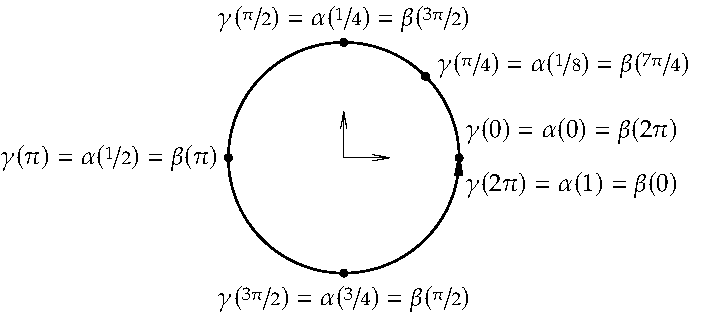
\includegraphics{figures/circlepathrepar}
\caption{A circular path reparametrized in two different ways. The arrow
indicates the orientation of $\gamma$ and $\alpha$. The path $\beta$ traverses
the circle in the
opposite direction.\label{fig:circlepathrepar}}
\end{myfigureht}
\end{example}

The previous example is not a fluke.
The path integral does not depend on the parametrization of
the curve, the only thing that matters is the direction in which the curve
is traversed.

\begin{prop} \label{mv:prop:pathintrepararam}
Let $\gamma \colon [a,b] \to \R^n$ be a piecewise smooth path and
$\gamma \circ h \colon [c,d] \to \R^n$ a piecewise smooth reparametrization.
Suppose $\omega$ is a one-form defined on the set $\gamma\bigl([a,b]\bigr)$.  Then
\begin{equation*}
\int_{\gamma \circ h} \omega =
\begin{cases}
\int_{\gamma} \omega  & \text{if } h \text{ preserves orientation,}\\
-\int_{\gamma} \omega & \text{if } h \text{ reverses orientation.}
\end{cases}
\end{equation*}
\end{prop}

\begin{proof}
Assume first that $\gamma$ and $h$ are both smooth.
Write $\omega = \omega_1 \, dx_1 + \omega_2 \, dx_2 + \cdots +
\omega_n \, dx_n$.
Suppose that $h$ is orientation preserving.  Use
the change of variables formula for the Riemann integral:
\begin{equation*}
\begin{split}
\int_{\gamma} \omega
& =
\int_a^b 
\left(
\sum_{j=1}^n
\omega_j\bigl(\gamma(t)\bigr) \gamma_j^{\:\prime}(t)
\right) dt
\\
& =
\int_c^d 
\left(
\sum_{j=1}^n
\omega_j\Bigl(\gamma\bigl(h(\tau)\bigr)\Bigr) \gamma_j^{\:\prime}\bigl(h(\tau)\bigr)
\right) h'(\tau) ~ d\tau
\\
& =
\int_c^d 
\left(
\sum_{j=1}^n
\omega_j\Bigl(\gamma\bigl(h(\tau)\bigr)\Bigr) (\gamma_j \circ h)'(\tau)
\right) d\tau
=
\int_{\gamma \circ h} \omega .
\end{split}
\end{equation*}
If $h$ is orientation reversing, it swaps the order of the limits on the
integral and introduces a minus sign.
The details, along with finishing the proof for piecewise smooth
paths, is left as \exerciseref{mv:exercise:pathpiece}.
\end{proof}

Due to this proposition (and the exercises), if $\Gamma
\subset \R^n$ is the image of a simple piecewise smooth path
$\gamma\bigl([a,b]\bigr)$, then as long as we somehow indicate the orientation, that
is, the direction in which we traverse the curve, we can write
\begin{equation*}
\int_{\Gamma} \omega ,
\end{equation*}
without mentioning the specific $\gamma$.
Furthermore, for a simple closed path, it does not even matter where we
start the parametrization.  See the exercises.

Recall that \emph{simple} means that $\gamma$
is one-to-one except perhaps at the endpoints, in particular
it is one-to-one when restricted to $[a,b)$.
We may relax the condition that the path is simple a little bit.
For example, it is enough to suppose that
$\gamma \colon [a,b] \to \R^n$ is one-to-one except at finitely many points.
%That is, there is a finite set $S \subset [a,b]$
%and $\gamma|_{[a,b]\setminus S}$ is one-to-one.
See \exerciseref{mv:exercise:curveintegral}.  But we cannot remove
the condition completely as is
illustrated by the following example.

\begin{example}
Suppose $\gamma \colon [0,2\pi] \to \R^2$ is given by $\gamma(t) :=
\bigl(\cos(t),\sin(t)\bigr)$, and
$\beta \colon [0,2\pi] \to \R^2$ is given by $\beta(t) :=
\bigl(\cos(2t),\sin(2t)\bigr)$.  Notice that
$\gamma\bigl([0,2\pi]\bigr) = \beta\bigl([0,2\pi]\bigr)$, and we travel
around the same curve, the unit circle.  But $\gamma$ goes around the unit
circle once in the counter clockwise direction, and $\beta$ goes around the
unit circle twice (in the same direction). 
See \figureref{fig:circlepathrepar2}.
\begin{myfigureht}
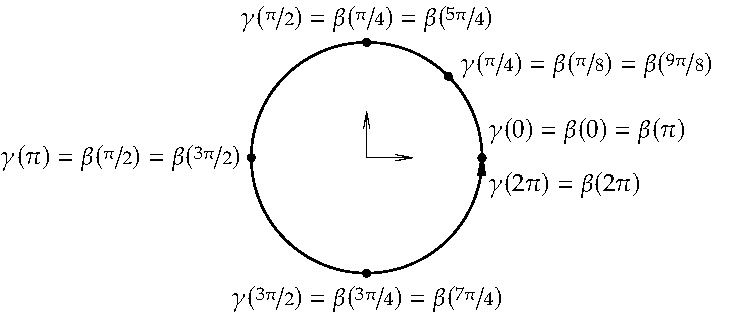
\includegraphics{figures/circlepathrepar2}
\caption{Circular path traversed once by
$\gamma \colon [0,2\pi] \to \R^2$
and twice by
$\beta \colon [0,2\pi] \to \R^2$.\label{fig:circlepathrepar2}}
\end{myfigureht}

Compute
\begin{align*}
& \int_{\gamma} -y~ dx + x~dy
=
\int_0^{2\pi}
\Bigl( \bigl(-\sin(t) \bigr) \bigl(-\sin(t) \bigr) + \cos(t) \cos(t) \Bigr) dt
=
2 \pi,\\
& \int_{\beta} -y~ dx + x~dy
=
\int_0^{2\pi}
\Bigl( \bigl(-\sin(2t) \bigr) \bigl(-2\sin(2t) \bigr) + \cos(t)
\bigl(2\cos(t)\bigr) \Bigr) dt
=
4 \pi.
\end{align*}
\end{example}

It is sometimes convenient to define a path integral over $\gamma \colon
[a,b] \to \R^n$ that is not a path.
Define
\glsadd{not:pathintegralomega}
\begin{equation*}
\int_{\gamma} \omega := \int_a^b
\left(
\sum_{j=1}^n
\omega_j\bigl(\gamma(t)\bigr) \gamma_j^{\:\prime}(t)
\right) dt 
\end{equation*}
for any continuously differentiable $\gamma$.  A 
case that comes up naturally is when $\gamma$ is constant.  Then
$\gamma^{\:\prime}(t) = 0$ for all $t$, and $\gamma\bigl([a,b]\bigr)$ is a single
point, which we regard as a \myquote{curve} of length zero.  Then,
$\int_{\gamma} \omega = 0$ for any $\omega$.

\subsection{Path integral of a function}

Next we integrate a function against the so-called
\emph{\myindex{arc-length measure}} $ds$.  The geometric picture we have in mind
is the area under the graph of the function over a path.
Imagine a fence erected over $\gamma$ with height given by the function
and the integral is the area of the fence.
See \figureref{fig:fenceintegral}.
\begin{myfigureht}
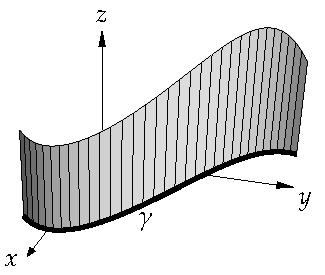
\includegraphics{figures/fenceintegral}
\caption{A path $\gamma \colon [a,b] \to \R^2$ in the $xy$-plane (bold curve), and a function
$z=f(x,y)$ graphed above it in the $z$ direction.  The integral is the
shaded area depicted.\label{fig:fenceintegral}}
\end{myfigureht}

\begin{defn}
Suppose $\gamma \colon [a,b] \to \R^n$ is a smooth path, and $f$ is a
continuous function defined on the image $\gamma\bigl([a,b]\bigr)$.  Then
define
\glsadd{not:lineintegralf}
\begin{equation*}
\int_{\gamma} f ~ds :=
\int_a^b f\bigl( \gamma(t) \bigr) \snorm{\gamma^{\:\prime}(t)} ~ dt .
\end{equation*}
To emphasize the variables we may use
\begin{equation*}
\int_{\gamma} f(x) ~ds(x) := \int_{\gamma} f ~ds .
\end{equation*}

The definition for a piecewise smooth path is similar as before and is left
to the reader.
\end{defn}

The path integral of a function is also independent of the parametrization,
and in this case, the orientation does not matter.

\begin{prop} \label{mv:prop:lineintrepararam}
Let $\gamma \colon [a,b] \to \R^n$ be a piecewise smooth path and
$\gamma \circ h \colon [c,d] \to \R^n$ a piecewise smooth reparametrization.
Suppose $f$ is a continuous function defined on the set
$\gamma\bigl([a,b]\bigr)$.  Then
\begin{equation*}
\int_{\gamma \circ h} f~ ds = \int_{\gamma} f~ ds .
\end{equation*}
\end{prop}

\begin{proof}
Suppose first that $h$ is orientation preserving and that $\gamma$ and $h$
are both smooth.  Then 
\begin{equation*}
\begin{split}
\int_{\gamma} f ~ ds
& =
\int_a^b 
f\bigl(\gamma(t)\bigr) \snorm{\gamma^{\:\prime}(t)} ~ dt
\\
& =
\int_c^d 
f\Bigl(\gamma\bigl(h(\tau)\bigr)\Bigr)
\snorm{\gamma^{\:\prime}\bigl(h(\tau)\bigr)} h'(\tau) ~ d\tau
\\
& =
\int_c^d 
f\Bigl(\gamma\bigl(h(\tau)\bigr)\Bigr)
\snorm{\gamma^{\:\prime}\bigl(h(\tau)\bigr) h'(\tau)} ~ d\tau
\\
& =
\int_c^d 
f\bigl((\gamma \circ h)(\tau)\bigr) \snorm{(\gamma \circ h)'(\tau)} ~ d\tau
\\
& = 
\int_{\gamma \circ h} f ~ ds .
\end{split}
\end{equation*}
If $h$ is orientation reversing it swaps the order of the limits on the
integral, but you also have to introduce a minus sign in order
to take $h'$ inside the norm.
The details, along with finishing the proof for piecewise smooth
paths is left to the reader as \exerciseref{mv:exercise:linepiece}.
\end{proof}

As before,
due to this proposition (and the exercises),
if $\gamma$ is simple, it does not matter which
parametrization we use.  Therefore, if $\Gamma = \gamma\bigl( [a,b] \bigr)$, we can
simply write
\begin{equation*}
\int_\Gamma f~ ds .
\end{equation*}
In this case we also do not need to worry about orientation, either way we
get the same integral.

\begin{example}
Let $f(x,y) := x$.  Let $C \subset \R^2$ be half of the unit circle for $x
\geq 0$.  We wish to compute
\begin{equation*}
\int_C f ~ ds .
\end{equation*}
Parametrize the curve $C$ via $\gamma \colon
[\nicefrac{-\pi}{2},\nicefrac{\pi}{2}] \to \R^2$ defined as
$\gamma(t) := \bigl(\cos(t),\sin(t)\bigr)$.
Then $\gamma^{\:\prime}(t) = \bigl(-\sin(t),\cos(t)\bigr)$, and
\begin{equation*}
\int_C f ~ ds =
\int_\gamma f ~ ds
=
\int_{-\pi/2}^{\pi/2} \cos(t) \sqrt{ {\bigl(-\sin(t)\bigr)}^2 +  
{\bigl(\cos(t)\bigr)}^2 } ~ dt
=
\int_{-\pi/2}^{\pi/2} \cos(t) ~ dt = 2.
\end{equation*}
\end{example}

\begin{defn}
Suppose $\Gamma \subset \R^n$ is parametrized by a simple
piecewise smooth path $\gamma \colon [a,b] \to \R^n$, that is
$\gamma\bigl( [a,b] \bigr) = \Gamma$.  We define the
\emph{\myindex{length}}\index{length of a curve} by
\begin{equation*}
\ell(\Gamma) := \int_{\Gamma} ds = \int_{\gamma} ds .
\end{equation*}
\end{defn}

If $\gamma$ is smooth,
\begin{equation*}
\ell(\Gamma) = 
\int_a^b
\snorm{\gamma^{\:\prime}(t)}~ dt .
\end{equation*}
This may be a good time to mention that it is common to write
$\int_a^b
\snorm{\gamma^{\:\prime}(t)}~ dt$ even if the path is only piecewise smooth.
That is because $\snorm{\gamma^{\:\prime}(t)}$ is defined and continuous
at all but finitely many points and is bounded, and so the integral exists.

\begin{example}
Let $x,y \in \R^n$ be two points and write $[x,y]$ as the straight line
segment between the two points $x$ and $y$.  Parametrize
$[x,y]$ by $\gamma(t) := (1-t)x + ty$ for $t$ running between $0$ and $1$.
See \figureref{fig:straightpath}.
Then $\gamma^{\:\prime}(t) = y-x$, and therefore
\begin{equation*}
\ell\bigl([x,y]\bigr)
=
\int_{[x,y]} ds
=
\int_0^1 \snorm{y-x} ~ dt
=
\snorm{y-x} .
\end{equation*}
So the length of $[x,y]$ is the standard euclidean distance between $x$ and $y$,
justifying the name.
\begin{myfigureht}
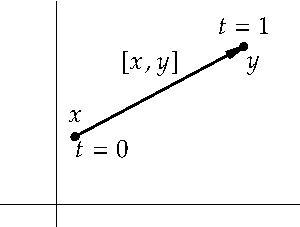
\includegraphics{figures/straightpath}
\caption{Straight path between $x$ and $y$ parametrized
by $(1-t)x + ty$.\label{fig:straightpath}}
\end{myfigureht}
\end{example}

A simple piecewise smooth path $\gamma \colon [0,r] \to \R^n$ is
said to be an \emph{\myindex{arc-length parametrization}} if
for all $t \in [0,r]$ we have
\begin{equation*}
\ell\bigl( \gamma\bigl([0,t]\bigr) \bigr) = t .
\end{equation*}
If $\gamma$ is smooth, then
\begin{equation*}
\int_0^t d\tau =
t = \ell\bigl( \gamma\bigl([0,t]\bigr) \bigr) =
\int_0^t
\snorm{\gamma^{\:\prime}(\tau)}
~ d\tau
\end{equation*}
for all $t$,
which means that $\snorm{\gamma^{\:\prime}(t)} = 1$ for all $t$.
Similarly for piecewise smooth $\gamma$, we get
$\snorm{\gamma^{\:\prime}(t)} = 1$ for all $t$ where the derivative exists.
So you can think of such a parametrization as moving around your curve at speed
1.  If $\gamma \colon [0,r] \to \R^n$ is an arclength parametrization, it is
common to use $s$ as the variable as $\int_\gamma f ~ds
= \int_0^r f\bigl(\gamma(s)\bigr) ~ds$.

\subsection{Exercises}

\begin{exercise}
Show that if $\varphi \colon [a,b] \to \R^n$ is a piecewise smooth path as we
defined it, then $\varphi$ is a continuous function.
\end{exercise}

\begin{exercise}
Finish the proof of \propref{prop:reparamapiecewisesmooth} for orientation
reversing reparametrizations.
\end{exercise}

\begin{exercise}
Prove \propref{mv:prop:pathconcat}.
\end{exercise}

\begin{exercise} \label{mv:exercise:pathpiece}
Finish the proof of \propref{mv:prop:pathintrepararam}
for
\begin{enumerate}[a)]
\item
orientation reversing reparametrizations, and
\item
piecewise smooth paths
and reparametrizations.
\end{enumerate}
\end{exercise}

\begin{exercise} \label{mv:exercise:linepiece}
Finish the proof of \propref{mv:prop:lineintrepararam}
for
\begin{enumerate}[a)]
\item
orientation reversing reparametrizations, and
\item
piecewise smooth paths
and reparametrizations.
\end{enumerate}
\end{exercise}

\begin{exercise}
Suppose $\gamma \colon [a,b] \to \R^n$ is a piecewise smooth path, and $f$ is a
continuous function defined on the image $\gamma\bigl([a,b]\bigr)$.
Provide a definition of $\int_{\gamma} f ~ds$.
\end{exercise}

\begin{exercise}
Directly using the definitions compute:
\begin{enumerate}[a)]
\item
The arc-length of the unit square from
\exampleref{mv:example:unitsquarepath} using the given parametrization.
\item
The arc-length of the unit circle using the parametrization
$\gamma \colon [0,1] \to \R^2$, $\gamma(t) := \bigl(\cos(2\pi t),\sin(2\pi t)\bigr)$.
\item
The arc-length of the unit circle using the parametrization
$\beta \colon [0,2\pi] \to \R^2$, $\beta(t) := \bigl(\cos(t),\sin(t)\bigr)$.
\end{enumerate}
Note: Feel free to use what you know about sine and cosine from calculus.
\end{exercise}

\begin{exercise}
Suppose $\gamma \colon [0,1] \to \R^n$ is a smooth path, and
$\omega$ is a one-form defined on the image $\gamma\bigl([a,b]\bigr)$.
For $r \in [0,1]$, let $\gamma_r \colon [0,r] \to \R^n$ be defined
as simply the restriction of $\gamma$ to $[0,r]$.  Show that the
function $h(r) := \int_{\gamma_r} \omega$ is a continuously
differentiable function on $[0,1]$.
\end{exercise}

\begin{exercise}
Suppose $\gamma \colon [a,b] \to \R^n$ is a smooth path.
Show that there exists an $\epsilon > 0$ and a smooth function
$\widetilde{\gamma} \colon (a-\epsilon,b+\epsilon) \to \R^n$
with $\widetilde{\gamma}(t) = \gamma(t)$ for all $t \in [a,b]$
and $\widetilde{\gamma}^{\:\prime}(t) \not= 0$ for all $t \in 
(a-\epsilon,b+\epsilon)$.  That is, prove that a smooth path extends
some small distance past the end points.
\end{exercise}

\begin{exercise} 
Suppose $\alpha \colon [a,b] \to \R^n$ and
$\beta \colon [c,d] \to \R^n$ are piecewise smooth paths such that
$\Gamma := \alpha\bigl([a,b]\bigr) = \beta\bigl([c,d]\bigr)$.
Show that there exist finitely many points
$\{ p_1,p_2,\ldots,p_k\} \in \Gamma$, such that
the sets
$\alpha^{-1}\bigl( \{ p_1,p_2,\ldots,p_k\} \bigr)$
and
$\beta^{-1}\bigl( \{ p_1,p_2,\ldots,p_k\} \bigr)$
are partitions of $[a,b]$ and $[c,d]$, such that on any subinterval
the paths are smooth (that is, they are partitions as in the definition
of piecewise smooth path).
\end{exercise}

\begin{exercise}
\leavevmode
\begin{enumerate}[a)]
\item
Suppose $\gamma \colon [a,b] \to \R^n$ and $\alpha \colon [c,d] \to \R^n$
are two smooth paths that are one-to-one and
$\gamma\bigl([a,b]\bigr) = \alpha\bigl([c,d]\bigr)$.  Then
there exists a smooth reparametrization $h \colon [a,b] \to [c,d]$
such that $\gamma = \alpha \circ h$.\\
Hint 1: It is not hard to show $h$ exists.
The trick is to prove it is continuously differentiable
with a nonzero derivative.  Apply the implicit function
theorem though it may at first seem the dimensions are wrong.\\
Hint 2: Worry about derivative of $h$ in $(a,b)$ first.
\item
Prove the same thing as part a, but now for simple closed paths with the
further assumption that $\gamma(a) = \gamma(b) = \alpha(c) = \alpha(d)$.
\item
Prove parts a) and b) but for piecewise smooth paths, obtaining
piecewise smooth reparametrizations.\\
Hint: The trick is to find two
partitions such that when restricted to a subinterval of the partition
both paths have the same image and are smooth, see the exercise above.
\end{enumerate}
\end{exercise}

\pagebreak[1]
\begin{exercise} 
Suppose $\alpha \colon [a,b] \to \R^n$ and
$\beta \colon [b,c] \to \R^n$ are piecewise smooth paths with
$\alpha(b)=\beta(b)$.  Let $\gamma \colon [a,c] \to \R^n$ be defined by
\begin{equation*}
\gamma(t) :=
\begin{cases}
\alpha(t) & \text{if } t \in [a,b], \\
\beta(t)  & \text{if } t \in (b,c].
\end{cases}
\end{equation*}
Show that $\gamma$ is a piecewise smooth path, and that if $\omega$ is a
one-form defined on the curve given by $\gamma$, then
\begin{equation*}
\int_{\gamma} \omega =
\int_{\alpha} \omega +
\int_{\beta} \omega .
\end{equation*}
\end{exercise}

\pagebreak[1]
\begin{exercise} \label{mv:exercise:closedcurveintegral}
Suppose $\gamma \colon [a,b] \to \R^n$ and
$\beta \colon [c,d] \to \R^n$ are two simple closed piecewise smooth paths.
That is, $\gamma(a)=\gamma(b)$ and $\beta(c) = \beta(d)$ and
the restrictions $\gamma|_{[a,b)}$ and $\beta|_{[c,d)}$ are one-to-one.
Suppose $\Gamma = \gamma\bigl([a,b]\bigr) = \beta\bigl([c,d]\bigr)$ and
$\omega$ is a one-form defined on $\Gamma \subset \R^n$.  Show that either
\begin{equation*}
\int_\gamma \omega = 
\int_\beta \omega,
\qquad \text{or} \qquad 
\int_\gamma \omega = 
- \int_\beta \omega.
\end{equation*}
In particular, the notation $\int_{\Gamma} \omega$ makes sense if we indicate
the direction in which the integral is evaluated.
Hint: See previous three exercises.
\end{exercise}

\begin{exercise} \label{mv:exercise:curveintegral}
Suppose $\gamma \colon [a,b] \to \R^n$ and
$\beta \colon [c,d] \to \R^n$ are two piecewise smooth paths
which are one-to-one except at finitely many points.  That is,
there exist finite sets $S \subset [a,b]$ and $T \subset [c,d]$
such that $\gamma|_{[a,b]\setminus S}$ and
$\beta|_{[c,d]\setminus T}$ are one-to-one.
Suppose $\Gamma = \gamma\bigl([a,b]\bigr) = \beta\bigl([c,d]\bigr)$ and $\omega$ is a
one-form defined on $\Gamma \subset \R^n$.  Show that either
\begin{equation*}
\int_\gamma \omega = 
\int_\beta \omega,
\qquad \text{or} \qquad 
\int_\gamma \omega = 
- \int_\beta \omega.
\end{equation*}
In particular, the notation $\int_{\Gamma} \omega$ makes sense if we indicate
the direction in which the integral is evaluated.
\\
Hint: Same hint as the last exercise.
\end{exercise}

\begin{exercise}
Define $\gamma \colon [0,1] \to \R^2$ by
$\gamma(t) := \Bigl( t^3 \sin(\nicefrac{1}{t}),\,
t{\bigl(3t^2\sin(\nicefrac{1}{t})-t\cos(\nicefrac{1}{t})\bigr)}^2 \Bigr)$
for
$t \not= 0$ and $\gamma(0) = (0,0)$.  Show that
\begin{enumerate}[a)]
\item
$\gamma$ is continuously differentiable on $[0,1]$.
\item
Show that there exists an infinite sequence $\{ t_n \}$ in $[0,1]$
converging to 0, such that
$\gamma^{\:\prime}(t_n) = (0,0)$.
\item
Show that the points $\gamma(t_n)$ lie on the line $y=0$ and such
that the $x$-coordinate of $\gamma(t_n)$ alternates between positive and
negative (if they do not alternate you only found a subsequence,
you need to find them all).
\item
Show that there is no piecewise smooth $\alpha$ whose image equals
$\gamma\bigl([0,1]\bigr)$.  Hint: Look at part c) and show that $\alpha'$
must be zero where it reaches the origin.
\item
(Computer) If you know a plotting software that allows you to plot
parametric curves, make a plot of the curve, but only for $t$ in the
range $[0,0.1]$ otherwise you will not see the behavior.  In particular, you
should notice that $\gamma\bigl([0,1]\bigr)$ has infinitely many
\myquote{corners}
near the origin.
\end{enumerate}
Note: Feel free to use what you know about sine and cosine from calculus.
\end{exercise}

%%%%%%%%%%%%%%%%%%%%%%%%%%%%%%%%%%%%%%%%%%%%%%%%%%%%%%%%%%%%%%%%%%%%%%%%%%%%%%

\sectionnewpage
\section{Path independence}
\label{sec:pathind}

\sectionnotes{2 lectures}

\subsection{Path independent integrals}

Let $U \subset \R^n$ be a set and $\omega$ a one-form defined on $U$.
The integral of $\omega$
is said to be \emph{\myindex{path independent}}
if for any two points $x,y \in U$ and
any two piecewise smooth paths
$\gamma \colon [a,b] \to U$ and
$\beta \colon [c,d] \to U$ such that $\gamma(a) = \beta(c) = x$
and $\gamma(b) = \beta(d) = y$ we have
\begin{equation*}
\int_\gamma \omega = \int_\beta \omega .
\end{equation*}
In this case, we simply write
\begin{equation*}
\int_x^y \omega := \int_\gamma \omega = \int_\beta \omega .
\end{equation*}
Not every one-form gives a path independent integral.  Most do not.

\begin{example}
Let $\gamma \colon [0,1] \to \R^2$ be the path $\gamma(t) := (t,0)$
going from $(0,0)$ to $(1,0)$.  Let $\beta \colon [0,1] \to \R^2$ be the path
$\beta(t) := \bigl(t,(1-t)t\bigr)$ also going between the same points.  Then
\begin{align*}
& \int_\gamma y ~ dx = 
\int_0^1 \gamma_2(t) \gamma_1^{\:\prime}(t) ~ dt
=
\int_0^1 0 (1) ~ dt = 0 ,\\
& \int_\beta y ~ dx = 
\int_0^1 \beta_2(t) \beta_1'(t) ~ dt
=
\int_0^1 (1-t)t(1) ~ dt = \frac{1}{6} .
\end{align*}
The integral of $y~dx$ is not path independent.
In particular,
$\int_{(0,0)}^{(1,0)} y~dx$ does not make sense.
\end{example}

\begin{defn}
Let $U \subset \R^n$ be an open set and $f \colon U \to \R$ a 
continuously differentiable function.  The one-form
\begin{equation*}
df :=
\frac{\partial f}{\partial x_1} ~ dx_1 + 
\frac{\partial f}{\partial x_2} ~ dx_2 + \cdots +
\frac{\partial f}{\partial x_n} ~ dx_n 
\end{equation*}
is called the \emph{\myindex{total derivative}} of $f$.

An open set $U \subset \R^n$ is said to be \emph{\myindex{path connected}}%
\footnote{Normally only a continuous path is used in this definition, but
for open sets the two definitions are equivalent.  See the exercises.}
if for every two points $x$ and $y$ in $U$, there exists a piecewise smooth
path starting at $x$ and ending at $y$.
\end{defn}

We leave as an exercise that every connected open set is path
connected.

\begin{prop} \label{mv:prop:pathinddf}
Let $U \subset \R^n$ be a path connected open set and $\omega$ a one-form
defined on $U$.  Then
$\int_x^y \omega$
is path independent (for all $x,y \in U$) if and only if there exists
a continuously differentiable $f \colon U \to \R$ such that $\omega = df$.

In fact, if such an $f$ exists, then for any two points $x,y \in U$
\begin{equation*}
\int_{x}^y \omega = f(y)-f(x) .
\end{equation*}
\end{prop}

In other words, if we fix $p \in U$, then $f(x) = C + \int_{p}^x \omega$
for some constant $C$.

\begin{proof}
First suppose that the integral is path independent.  Pick $p \in U$.  Since
$U$ is path connected, there exists a path from $p$ to any $x \in U$.
Define
\begin{equation*}
f(x) := \int_{p}^x \omega .
\end{equation*}
Write $\omega = \omega_1 \,dx_1 + \omega_2 \,dx_2 + \cdots + \omega_n \,dx_n$.
We wish to show that for every $j = 1,2,\ldots,n$, the
partial derivative $\frac{\partial f}{\partial x_j}$ exists
and is equal to $\omega_j$.

Let $e_j$ be an arbitrary standard basis vector, and $h$ a nonzero real
number.  Compute
\begin{equation*}
\frac{f(x+h e_j) - f(x)}{h} =
\frac{1}{h} \left( \int_{p}^{x+he_j} \omega - \int_{p}^x \omega \right)
=
\frac{1}{h} \int_{x}^{x+he_j} \omega ,
\end{equation*}
which follows by \propref{mv:prop:pathconcat} and path independence as 
$\int_{p}^{x+he_j} \omega =
\int_{p}^{x} \omega +
\int_{x}^{x+he_j} \omega$, because we pick a path from $p$ to
$x+he_j$ that also happens to pass through $x$, and then we cut this path in
two, see \figureref{fig:pathindantider}.

\begin{myfigureht}
\subimport*{figures/}{pathindantider.pdf_t}
\caption{Using path independence in computing the partial
derivative.\label{fig:pathindantider}}
\end{myfigureht}


Since $U$ is open, suppose $h$ is so small so that all points of distance
$\abs{h}$ or
less from $x$ are in $U$.
As the integral is path independent,
pick the simplest path possible from $x$ to $x+he_j$, that is
$\gamma(t) := x+t he_j$ for $t \in [0,1]$.  The path is in $U$.
Notice $\gamma^{\:\prime}(t) = h e_j$
has only one nonzero component and that is the $j$th component, which is
$h$.  Therefore
\begin{equation*}
\frac{1}{h} \int_{x}^{x+he_j} \omega 
=
\frac{1}{h} \int_{\gamma} \omega 
=
\frac{1}{h} \int_0^1 \omega_j(x+the_j) h ~ dt 
=
\int_0^1 \omega_j(x+the_j) ~ dt  .
\end{equation*}
We wish to take the limit as $h \to 0$.  The function $\omega_j$ is
continuous at $x$.  Given $\epsilon > 0$, suppose $h$ is small enough so that
$\abs{\omega(x)-\omega(y)} < \epsilon$, whenever $\snorm{x-y} \leq \abs{h}$.
Hence,
$\abs{\omega_j(x+the_j)-\omega_j(x)} < \epsilon$ for all $t \in [0,1]$,
and we estimate
\begin{equation*}
\abs{\int_0^1 \omega_j(x+the_j) ~ dt  - \omega(x)}
=
\abs{\int_0^1 \bigl( \omega_j(x+the_j) - \omega(x) \bigr) ~ dt}
\leq
\epsilon .
\end{equation*}
That is,
\begin{equation*}
\lim_{h\to 0}\frac{f(x+h e_j) - f(x)}{h} = \omega_j(x) .
\end{equation*}
All partials of $f$ exist and are equal to $\omega_j$, which are continuous
functions.  Thus, $f$ is continuously differentiable, and furthermore
$df = \omega$.

For the other direction,
suppose a continuously differentiable $f$ exists such that $df = \omega$.
Take a smooth
path
$\gamma \colon [a,b] \to U$ such that $\gamma(a) = x$ and
$\gamma(b) = y$.  Then
\begin{equation*}
\begin{split}
\int_\gamma df
& =
\int_a^b
\biggl(
\frac{\partial f}{\partial x_1}\bigl(\gamma(t)\bigr) \gamma_1^{\:\prime}(t)+
\frac{\partial f}{\partial x_2}\bigl(\gamma(t)\bigr) \gamma_2^{\:\prime}(t)+ \cdots +
\frac{\partial f}{\partial x_n}\bigl(\gamma(t)\bigr) \gamma_n^{\:\prime}(t)
\biggr) ~ dt
\\
& = 
\int_a^b
\frac{d}{dt} \Bigl[ f\bigl(\gamma(t)\bigr) \Bigr]~ dt
\\
& = f(y)-f(x) .
\end{split}
\end{equation*}
The value of the integral only depends on $x$ and $y$, not the
path taken.  Therefore the integral is path independent.
We leave checking this fact for a piecewise smooth path as an exercise.
\end{proof}

Path independence can be stated more neatly in terms of integrals over
closed paths.

\begin{prop}
Let $U \subset \R^n$ be a path connected open set and $\omega$
a one-form defined on $U$.
Then $\omega = df$ for some continuously differentiable $f \colon U \to
\R$ if and only if
\begin{equation*}
\int_{\gamma} \omega = 0
\qquad
\text{for every piecewise smooth closed path } \gamma \colon [a,b] \to U.
\end{equation*}
\end{prop}

\begin{proof}
Suppose $\omega = df$ and let $\gamma$ be a piecewise smooth
closed path.  
Since $\gamma(a) = \gamma(b)$ for a closed path,
the previous proposition says
\begin{equation*}
\int_{\gamma} \omega = f\bigl(\gamma(b)\bigr) - f\bigl(\gamma(a)\bigr) = 0 .
\end{equation*}

Now suppose that for every piecewise smooth closed path $\gamma$, $\int_{\gamma} \omega = 0$.
Let $x,y$ be two points in $U$ and let $\alpha \colon [0,1] \to U$ and
$\beta \colon [0,1] \to U$ be two piecewise smooth paths with $\alpha(0) = \beta(0) = x$
and $\alpha(1) = \beta(1) = y$.  See \figureref{fig:twopaths}.
\begin{myfigureht}
\subimport*{figures/}{twopaths.pdf_t}
\caption{Two paths from $x$ to $y$.\label{fig:twopaths}}
\end{myfigureht}

Define $\gamma \colon [0,2] \to U$ by
\begin{equation*}
\gamma(t) :=
\begin{cases}
\alpha(t)  & \text{if } t \in [0,1], \\
\beta(2-t) & \text{if } t \in (1,2].
\end{cases}
\end{equation*}
This path is piecewise smooth.  This is due to the fact that
$\gamma|_{[0,1]}(t) = \alpha(t)$ and
$\gamma|_{[1,2]}(t) = \beta(2-t)$ (note especially $\gamma(1) = \alpha(1) =
\beta(2-1)$).
It is also closed as $\gamma(0) = \alpha(0) = \beta(0) = \gamma(2)$.
So 
\begin{equation*}
0 = \int_{\gamma} \omega = \int_{\alpha} \omega - \int_{\beta} \omega .
\end{equation*}
This follows first by \propref{mv:prop:pathconcat}, and then noticing that
the second part is $\beta$ traveled backwards so that we get minus the
$\beta$ integral.  Thus the integral of $\omega$ on $U$ is path independent.
\end{proof}

However one states path independence, it is often a difficult criterion to
check, you have to check something \myquote{for all paths.}
There is a local criterion, a differential equation, that guarantees
path independence, or in other words it guarantees an
\emph{\myindex{antiderivative}}
$f$ whose total derivative is the given one-form
$\omega$.  Since the criterion is local, we generally only find the
function $f$ locally.
We can find the antiderivative in any so-called
\emph{\myindex{simply connected}} domain, which informally is a domain where
any path between two points can be \myquote{continuously deformed}
into any other path
between those two points.  But to make matters simple, we prove
the result for so-called star-shaped domains, which is often good enough.
As a bonus the proof in the star-shaped case constructs
the antiderivative explicitly.
As balls are star-shaped we then have the result locally.

\begin{defn}
Let $U \subset \R^n$ be an open set and $p \in U$.  We say $U$ is
a \emph{\myindex{star-shaped domain}}
with respect to $p$ if for any other point $x \in U$,
the line segment $[p,x]$ is in $U$, that is, if
$(1-t)p + tx \in U$ for all $t \in [0,1]$.
If we say simply \emph{star-shaped}, then $U$ is star-shaped with respect to
some $p \in U$.  See \figureref{fig:starshaped}.
\begin{myfigureht}
\subimport*{figures/}{starshaped.pdf_t}
\caption{A star-shaped domain with respect to $p$.\label{fig:starshaped}}
\end{myfigureht}
\end{defn}

Notice the difference between star-shaped and convex.  A convex domain is
star-shaped, but a star-shaped domain need not be convex.

\begin{thm}[\myindex{Poincar\'e lemma}]
Let $U \subset \R^n$ be a star-shaped domain and $\omega$ a continuously
differentiable one-form defined on $U$.  That is, if
\begin{equation*}
\omega =
\omega_1 \,dx_1 +
\omega_2 \,dx_2 + \cdots +
\omega_n \,dx_n ,
\end{equation*}
then $\omega_1,\omega_2,\ldots,\omega_n$ are continuously differentiable
functions.  Suppose that for every $j$ and $k$
\begin{equation*}
\frac{\partial \omega_j}{\partial x_k} = \frac{\partial \omega_k}{\partial x_j} ,
\end{equation*}
then there exists a twice continuously differentiable function $f \colon U
\to \R$
such that $df = \omega$.
\end{thm}

The condition on the derivatives of $\omega$ is precisely the condition
that the second partial derivatives commute.  That is, if $df = \omega$,
and $f$ is twice continuously differentiable, then
\begin{equation*}
\frac{\partial \omega_j}{\partial x_k}
=
\frac{\partial^2 f}{\partial x_k \partial x_j} 
=
\frac{\partial^2 f}{\partial x_j \partial x_k} 
=
\frac{\partial \omega_k}{\partial x_j} .
\end{equation*}
The condition is clearly necessary.  The Poincar\'e lemma says that it is
sufficient for a star-shaped $U$.

\begin{proof}
Suppose $U$ is a star-shaped domain with respect to $p=(p_1,p_2,\ldots,p_n) \in U$.
Given $x = (x_1,x_2,\ldots,x_n) \in U$, define the path $\gamma \colon [0,1] \to U$ as
$\gamma(t) := (1-t)p + tx$, so $\gamma^{\:\prime}(t) = x-p$.  Let
\begin{equation*}
f(x) := \int_{\gamma} \omega
=
\int_0^1
\left(
\sum_{k=1}^n
\omega_k \bigl((1-t)p + tx \bigr) \, (x_k-p_k)
\right) dt .
\end{equation*}
We differentiate in $x_j$ under the integral, which is allowed as
everything, including the partials, is continuous:
\begin{equation*}
\begin{split}
\frac{\partial f}{\partial x_j}(x) & =
\int_0^1
\left(
\left(
\sum_{k=1}^n
\frac{\partial \omega_k}{\partial x_j} \bigl((1-t)p + tx \bigr) \, t
(x_k-p_k)
\right)
+
\omega_j \bigl((1-t)p + tx \bigr)
\right)
 dt
\\
& = 
\int_0^1
\left(
\left(
\sum_{k=1}^n
\frac{\partial \omega_j}{\partial x_k} \bigl((1-t)p + tx \bigr) \, t
(x_k-p_k)
\right)
+
\omega_j \bigl((1-t)p + tx \bigr)
\right) dt
\\
& = 
\int_0^1
\frac{d}{dt}
\Bigl[
t \omega_j\bigl((1-t)p + tx \bigr)
\Bigr]
\,
dt
\\
&= \omega_j(x) .
\end{split}
\end{equation*}
And this is precisely what we wanted.
\end{proof}

\begin{example}
Without some hypothesis on $U$ the theorem is not true.  Let
\begin{equation*}
\omega(x,y) := \frac{-y}{x^2+y^2} ~dx + \frac{x}{x^2+y^2} ~dy
\end{equation*}
be defined on $\R^2 \setminus \{ 0 \}$.  Then
\begin{equation*}
\frac{\partial}{\partial y} \left[ 
\frac{-y}{x^2+y^2} \right] =
\frac{y^2-x^2}{{(x^2+y^2)}^2}
=
\frac{\partial}{\partial x} \left[ 
\frac{x}{x^2+y^2} \right] .
\end{equation*}
However, there is no $f \colon \R^2 \setminus \{ 0 \} \to \R$ such that 
$df = \omega$.  In
\exampleref{example:mv:irrotoneformint} we integrated from $(1,0)$ to $(1,0)$
along the unit circle counterclockwise,
that is $\gamma(t) = \bigl(\cos(t),\sin(t)\bigr)$
for $t \in [0,2\pi]$, and we found the integral to be $2\pi$.  We would have
gotten $0$ if
the integral was path independent,
or in other words if there would exist an $f$ such that
$df = \omega$.
\end{example}

\subsection{Vector fields}

A common object to integrate is a so-called vector field.

\begin{defn}
Let $U \subset \R^n$ be a set.
A continuous function $v \colon U \to \R^n$ is called a
\emph{\myindex{vector field}}.  Write $v = (v_1,v_2,\ldots,v_n)$.

Given a smooth path $\gamma \colon [a,b] \to \R^n$ with
$\gamma\bigl([a,b]\bigr) \subset U$ we define
the path integral of the vectorfield $v$ as
\glsadd{not:pathintegralvecfield}
\begin{equation*}
\int_{\gamma} v \cdot d\gamma
:=
\int_a^b v\bigl(\gamma(t)\bigr) \cdot \gamma^{\:\prime}(t) ~ dt ,
\end{equation*}
where the dot in the definition is the standard dot product.
The definition for a piecewise smooth path is, again, done by integrating over
each smooth interval and adding the results.
\end{defn}

Unraveling the definition, we find that
\begin{equation*}
\int_{\gamma} v \cdot d\gamma
=
\int_{\gamma} v_1 ~dx_1 + v_2 ~dx_2 + \cdots + v_n ~dx_n .
\end{equation*}
What we know about integration of
one-forms carries over to the integration of vector fields.
For example, path independence for integration of vector fields is simply
that
\begin{equation*}
\int_x^y v \cdot d\gamma
\end{equation*}
is path independent if and only if 
$v = \nabla f$, that is, $v$ is the gradient of a function.  The function $f$
is then called a \emph{\myindex{potential}} for $v$.

A vector field $v$ whose path integrals are path independent is called
a \emph{\myindex{conservative vector field}}.  The rationale for the naming
is that such vector fields arise in physical systems
where a certain quantity, the energy, is conserved.

\subsection{Exercises}

\begin{exercise}
Find an $f \colon \R^2 \to \R$ such that $df = xe^{x^2+y^2}\, dx +
ye^{x^2+y^2} \, dy$.
\end{exercise}

\begin{exercise}
Find an $\omega_2 \colon \R^2 \to \R$ such that
there exists a continuously differentiable $f \colon \R^2 \to \R$
for which
$df = e^{xy} ~dx + \omega_2 ~dy$.
\end{exercise}

\begin{exercise}
Finish the proof of \propref{mv:prop:pathinddf}, that is, we only proved the
second direction for a smooth path, not a piecewise smooth path.
\end{exercise}

\begin{exercise}
Show that a star-shaped domain $U \subset \R^n$ is path connected.
\end{exercise}

\begin{exercise}
Show that $U := \R^2 \setminus \{ (x,y) \in \R^2 : x \leq 0, y=0 \}$ is
star-shaped and find all points $(x_0,y_0) \in U$ such that
$U$ is star-shaped with respect to $(x_0,y_0)$.
\end{exercise}

\begin{exercise}
Suppose $U_1$ and $U_2$ are two open sets in $\R^n$ with $U_1 \cap U_2$
nonempty and path connected.
Suppose there exists an $f_1 \colon U_1 \to \R$ and
$f_2 \colon U_2 \to \R$, both twice continuously differentiable
such that $d f_1 = d f_2$ on $U_1 \cap U_2$.
Then there exists a twice differentiable function $F \colon U_1 \cup U_2 \to
\R$ such that $dF = df_1$ on $U_1$ and $dF = df_2$ on $U_2$.
\end{exercise}

\begin{exercise}[Hard]
Let $\gamma \colon [a,b] \to \R^n$ be a simple nonclosed piecewise smooth
path (so $\gamma$
is one-to-one).  Suppose $\omega$ is a continuously differentiable
one-form defined on some open
set $V$ with $\gamma\bigl([a,b]\bigr) \subset V$ and
$\frac{\partial \omega_j}{\partial x_k} = \frac{\partial \omega_k}{\partial
x_j}$
for all $j$ and $k$.  Prove that there exists an open set $U$
with $\gamma\bigl([a,b]\bigr) \subset U \subset V$ and
a twice continuously differentiable function $f \colon U \to \R$
such that $df = \omega$.
\\
Hint 1: $\gamma\bigl([a,b]\bigr)$ is compact.\\
Hint 2: Show that you can cover the curve by finitely many balls in sequence
so that the $k$th ball only intersects the $(k-1)$th ball.\\
Hint 3: See previous exercise.
\end{exercise}

\pagebreak[2]
\begin{exercise}
\leavevmode
\begin{enumerate}[a)]
\item
Show that a connected open set $U \subset \R^n$ is path connected.
Hint: Start with a
point $x \in U$, and let $U_x \subset U$ is the set of points that are
reachable by a path from $x$.  Show that $U_x$ and $U \setminus U_x$
are both open, and since $U_x$ is nonempty ($x \in U_x$) it must be
that $U_x = U$.
\item
Prove the converse, that is, an open\footnote{If the
definition of \myquote{path connected} is as in the next exercise,
\myquote{open} would not be needed for this part.}
path connected set $U \subset \R^n$ is
connected.  Hint: For contradiction assume there exist two open and disjoint nonempty open
sets and then assume there is a piecewise smooth (and therefore continuous)
path between a point in one to a point in the other.
\end{enumerate}
\end{exercise}

\begin{exercise}
Usually path connectedness is defined using continuous paths rather
than piecewise smooth paths.  Prove that for open subsets of $\R^n$
the definitions are equivalent, in
other words prove:\\
Suppose $U \subset \R^n$ is open and for any $x,y \in U$, there exists a continuous function
$\gamma \colon [a,b] \to U$ such that $\gamma(a) = x$ and $\gamma(b) = y$.
Then $U$ is path connected, that is, there is a piecewise smooth path in $U$ from
$x$ to $y$.
\end{exercise}

\begin{exercise}[Hard]
Take
\begin{equation*}
\omega(x,y) = \frac{-y}{x^2+y^2} \, dx + \frac{x}{x^2+y^2} \, dy
\end{equation*}
defined on $\R^2 \setminus \{ (0,0) \}$.  Let $\gamma \colon [a,b] \to \R^2
\setminus \{ (0,0) \}$ be a closed piecewise smooth path.
Let $R:=\{ (x,y) \in \R^2 : x \leq 0 \text{ and } y=0 \}$.
Suppose $R \cap \gamma\bigl([a,b]\bigr)$ is a finite set of $k$ points.
Prove that
\begin{equation*}
\int_{\gamma} \omega = 2 \pi \ell 
\end{equation*}
for some integer $\ell$ with $\abs{\ell} \leq k$.\\
Hint 1: First prove that for a path $\beta$ that starts and end on $R$ but
does not intersect it otherwise, you find that $\int_{\beta} \omega$
is $-2\pi$, 0, or $2\pi$.
\\
Hint 2: You proved above that $\R^2 \setminus R$ is star-shaped.
\\
Note: The number $\ell$ is called the \emph{\myindex{winding number}} it measures how many
times does $\gamma$ wind around the origin in the clockwise direction.
\end{exercise}
